\documentclass[11pt,a4paper]{report}
\usepackage[textwidth=37em,vmargin=30mm]{geometry}
\usepackage{calc,xunicode,amsmath,amssymb,paralist,enumitem,tabu,booktabs,datetime2,xeCJK,xeCJKfntef,listings}
\usepackage{tocloft,fancyhdr,tcolorbox,xcolor,graphicx,eso-pic,xltxtra,xelatexemoji}

\newcommand{\envyear}[0]{2025}
\newcommand{\envdatestr}[0]{2025-04-11}
\newcommand{\envfinaldir}[0]{webdb/2025/20250411/final}

\usepackage[hidelinks]{hyperref}
\hypersetup{
    colorlinks=false,
    pdfpagemode=FullScreen,
    pdftitle={Web Digest - \envdatestr}
}

\setlength{\cftbeforechapskip}{10pt}
\renewcommand{\cftchapfont}{\rmfamily\bfseries\large\raggedright}
\setlength{\cftbeforesecskip}{2pt}
\renewcommand{\cftsecfont}{\sffamily\small\raggedright}

\setdefaultleftmargin{2em}{2em}{1em}{1em}{1em}{1em}

\usepackage{xeCJK,xeCJKfntef}
\xeCJKsetup{PunctStyle=plain,RubberPunctSkip=false,CJKglue=\strut\hskip 0pt plus 0.1em minus 0.05em,CJKecglue=\strut\hskip 0.22em plus 0.2em}
\XeTeXlinebreaklocale "zh"
\XeTeXlinebreakskip = 0pt


\setmainfont{Brygada 1918}
\setromanfont{Brygada 1918}
\setsansfont{IBM Plex Sans}
\setmonofont{JetBrains Mono NL}
\setCJKmainfont{Noto Serif CJK SC}
\setCJKromanfont{Noto Serif CJK SC}
\setCJKsansfont{Noto Sans CJK SC}
\setCJKmonofont{Noto Sans CJK SC}

\setlength{\parindent}{0pt}
\setlength{\parskip}{8pt}
\linespread{1.15}

\lstset{
	basicstyle=\ttfamily\footnotesize,
	numbersep=5pt,
	backgroundcolor=\color{black!5},
	showspaces=false,
	showstringspaces=false,
	showtabs=false,
	tabsize=2,
	captionpos=b,
	breaklines=true,
	breakatwhitespace=true,
	breakautoindent=true,
	linewidth=\textwidth
}






\newcommand{\coverpic}[2]{
    % argv: itemurl, authorname
    Cover photo by #2~~(\href{#1}{#1})
}
\newcommand{\makeheader}[0]{
    \begin{titlepage}
        % \newgeometry{hmargin=15mm,tmargin=21mm,bmargin=12mm}
        \begin{center}
            
            \rmfamily\scshape
            \fontspec{BaskervilleF}
            \fontspec{Old Standard}
            \fontsize{59pt}{70pt}\selectfont
            WEB\hfill DIGEST
            
            \vfill
            % \vskip 30pt
            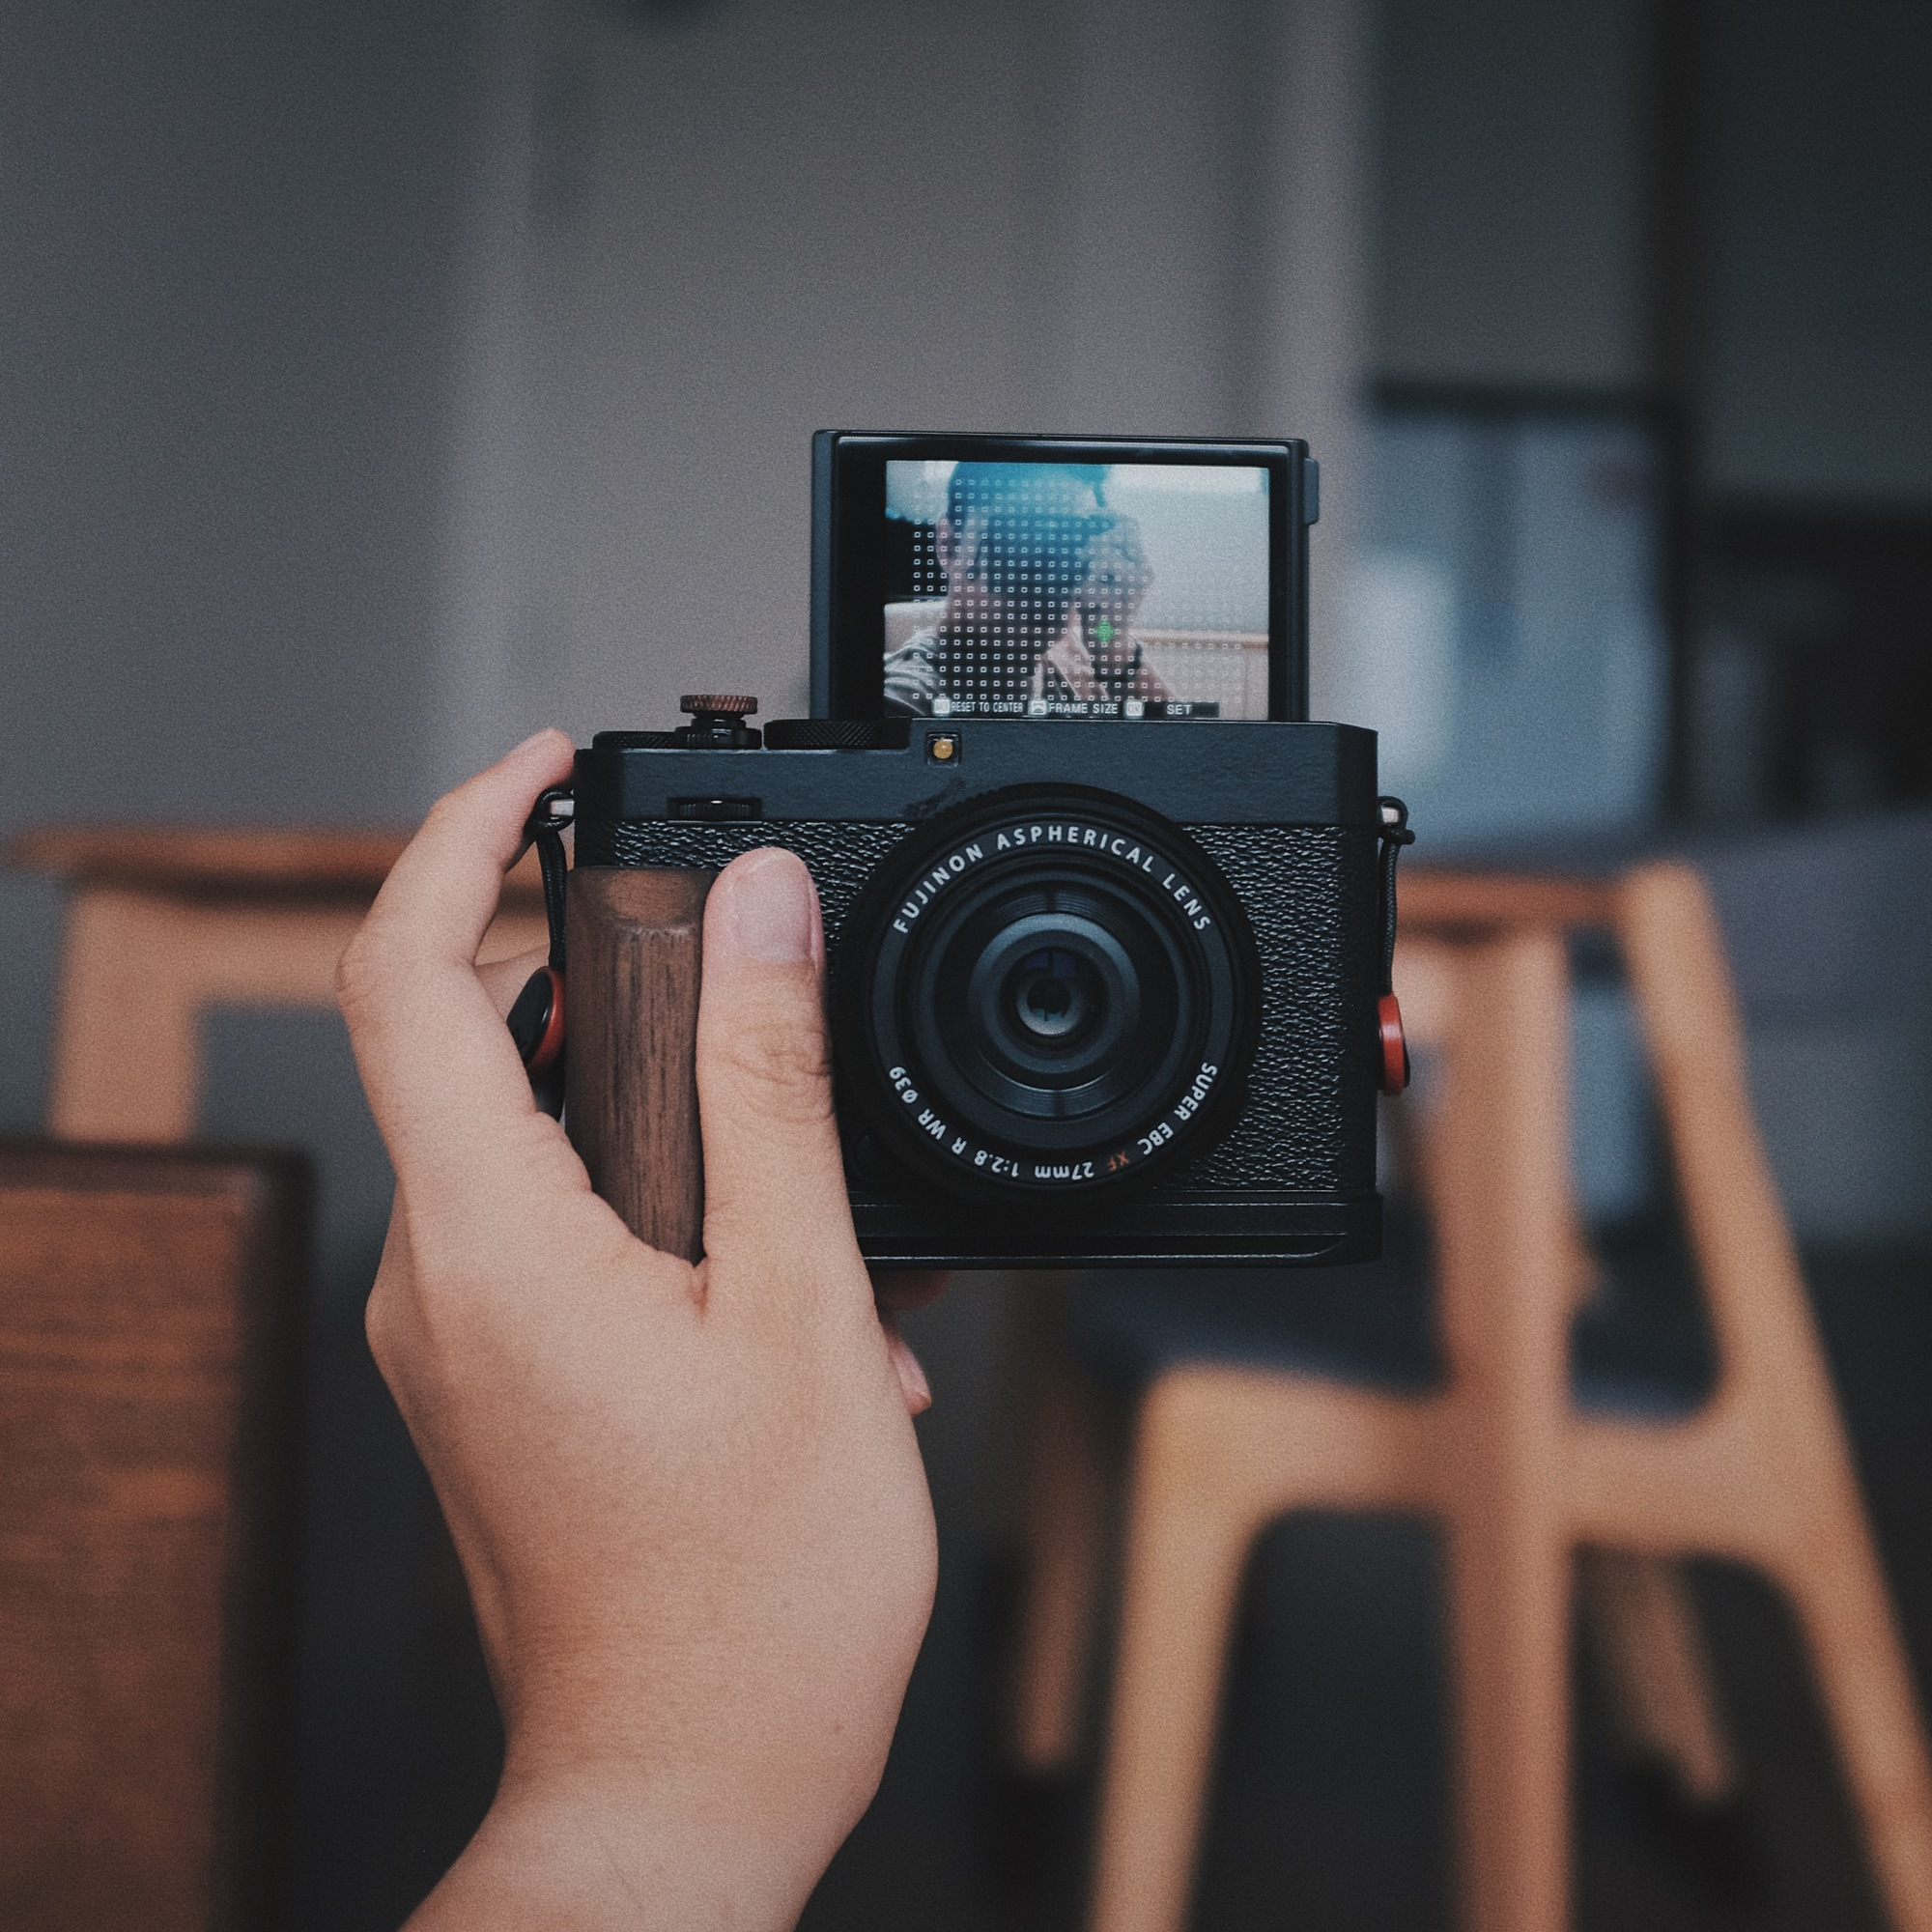
\includegraphics[width=\linewidth]{\envfinaldir/coverpic-prod.jpg}\par
            % \vskip 30pt
            \vfill

            \normalsize\rmfamily\scshape
            \copyright{} The Web Digest Project \hfill\large \envdatestr
        \end{center}
    \end{titlepage}
    % \restoregeometry
}
\newcommand{\simplehref}[1]{%
    \textcolor{blue!80!green}{\href{#1}{#1}}%
}
\renewcommand{\contentsname}{\center\Huge\sffamily\bfseries Contents\par\vskip 20pt}
\newcounter{ipartcounter}
\setcounter{ipartcounter}{0}
\newcommand{\ipart}[1]{
    % \vskip 20pt
    \clearpage
    \stepcounter{ipartcounter}
    \phantomsection
    \addcontentsline{toc}{chapter}{#1}
    % \begin{center}
    %     \Huge
    %     \sffamily\bfseries
    %     #1
    % \end{center}
    % \vskip 20pt plus 7pt
}
\newcounter{ichaptercounter}
\setcounter{ichaptercounter}{0}
\newcommand{\ichapter}[1]{
    % \vskip 20pt
    \clearpage
    \stepcounter{ichaptercounter}
    \phantomsection
    \addcontentsline{toc}{section}{\numberline{\arabic{ichaptercounter}}#1}
    \begin{center}
        \Huge
        \sffamily\bfseries
        #1
    \end{center}
    \vskip 20pt plus 7pt
}
\newcommand{\entrytitlefont}[1]{\subsection*{\raggedright\Large\sffamily\bfseries#1}}
\newcommand{\entryitemGeneric}[2]{
    % argv: title, url
    \parbox{\linewidth}{
        \entrytitlefont{#1}\par\vskip 5pt
        \footnotesize\ttfamily\mdseries
        \simplehref{#2}
    }\vskip 11pt plus 11pt minus 1pt
}
\newcommand{\entryitemGithub}[3]{
    % argv: title, url, desc
    \parbox{\linewidth}{
        \entrytitlefont{#1}\par\vskip 5pt
        \footnotesize\ttfamily\mdseries
        \simplehref{#2}\par\vskip 5pt
        \small\rmfamily\mdseries#3
    }\vskip 11pt plus 11pt minus 1pt
}
\newcommand{\entryitemAp}[3]{
    % argv: title, url, desc
    \parbox{\linewidth}{
        \entrytitlefont{#1}\par\vskip 5pt
        \footnotesize\ttfamily\mdseries
        \simplehref{#2}\par\vskip 5pt
        \small\rmfamily\mdseries#3
    }\vskip 11pt plus 11pt minus 1pt
}
\newcommand{\entryitemHackernews}[3]{
    % argv: title, hnurl, rawurl
    % \parbox{\linewidth}{
    %     \entrytitlefont{#1}\par\vskip 5pt
    %     \footnotesize\ttfamily\mdseries
    %     \simplehref{#3}\par
    %     \textcolor{black!50}{\href{#2}{#2}}
    % }\vskip 11pt plus 11pt minus 1pt
    \begin{minipage}{\linewidth}
            \entrytitlefont{#1}\par\vskip 5pt
            \footnotesize\ttfamily\mdseries
            \simplehref{#3}\par
            \textcolor{black!50}{\href{#2}{#2}}
    \end{minipage}\par\vskip 11pt plus 11pt minus 1pt
}







\begin{document}

\makeheader

\tableofcontents\clearpage




\ipart{Developers}
\ichapter{Hacker News}
\entryitemTwoLinks{So, I Wrote a Book: The Story Behind ``100 Go Mistakes and How to Avoid Them''}{https://news.ycombinator.com/item?id=43647880}{https://www.thecoder.cafe/p/100-go-mistakes}

\entryitemTwoLinks{PEP 750 – Template Strings (t-strings) have been accepted}{https://news.ycombinator.com/item?id=43647716}{https://peps.python.org/pep-0750/}

\entryitemTwoLinks{Big Book of R}{https://news.ycombinator.com/item?id=43646219}{https://www.bigbookofr.com/}

\entryitemTwoLinks{Garfield Minus Garfield}{https://news.ycombinator.com/item?id=43646095}{https://garfieldminusgarfield.net}

\entryitemTwoLinks{Why Tap a Wheel of Cheese?}{https://news.ycombinator.com/item?id=43644970}{https://www.cheeseprofessor.com/blog/cheese-wheel-tapping}

\entryitemTwoLinks{Isaac Asimov describes how AI will liberate humans and their creativity (1992)}{https://news.ycombinator.com/item?id=43644179}{https://www.openculture.com/2025/04/isaac-asimov-describes-how-ai-will-liberate-humans-their-creativity.html}

\entryitemTwoLinks{.localhost Domains}{https://news.ycombinator.com/item?id=43644043}{https://inclouds.space/localhost-domains}

\entryitemTwoLinks{Usability Improvements in GCC 15}{https://news.ycombinator.com/item?id=43643886}{https://developers.redhat.com/articles/2025/04/10/6-usability-improvements-gcc-15}

\entryitemTwoLinks{Busy Bar}{https://news.ycombinator.com/item?id=43643534}{https://busy.bar}

\entryitemTwoLinks{Sleep is essential – researchers are trying to work out why}{https://news.ycombinator.com/item?id=43643390}{https://www.nature.com/articles/d41586-025-00964-w}

\entryitemTwoLinks{Owning my own data, part 1: Integrating a self-hosted calendar solution}{https://news.ycombinator.com/item?id=43643343}{https://emilygorcenski.com/post/owning-my-own-data-part-1-integrating-a-self-hosted-calendar-solution/}

\entryitemTwoLinks{Elliptical Python Programming}{https://news.ycombinator.com/item?id=43643292}{https://susam.net/elliptical-python-programming.html}

\entryitemTwoLinks{America Is Backsliding Toward Its Most Polluted Era}{https://news.ycombinator.com/item?id=43643243}{https://www.theatlantic.com/health/archive/2025/04/air-pollution-trump-administration/682361/}

\entryitemTwoLinks{Hacker News Hug of Deaf}{https://news.ycombinator.com/item?id=43642123}{https://susam.net/hn-bell.html}

\entryitemTwoLinks{Hunt for Red October 1990 (2016)}{https://news.ycombinator.com/item?id=43641469}{http://www.modelshipsinthecinema.com/2016/12/hunt-for-red-october-1990.html}

\entryitemTwoLinks{ICE director envisions Amazon-like mass deportation system}{https://news.ycombinator.com/item?id=43641402}{https://azmirror.com/2025/04/08/ice-director-envisions-amazon-like-mass-deportation-system-prime-but-with-human-beings/}

\entryitemTwoLinks{Learning to Program with Haiku}{https://news.ycombinator.com/item?id=43640403}{https://www.haiku-os.org/development/learning\_to\_program\_with\_haiku}

\entryitemTwoLinks{NIH freezes all research grants to Columbia University}{https://news.ycombinator.com/item?id=43640267}{https://www.science.org/content/article/nih-freezes-all-research-grants-columbia-university}

\entryitemTwoLinks{No Pay, No Work; Early Career Lessons}{https://news.ycombinator.com/item?id=43639871}{https://danielsada.tech/blog/carreer-part-3-no-pay-no-work/}

\entryitemTwoLinks{Colossus for Rapid Storage}{https://news.ycombinator.com/item?id=43639642}{https://cloud.google.com/blog/products/storage-data-transfer/how-the-colossus-stateful-protocol-benefits-rapid-storage}\ichapter{Phoronix}
\entryitemGeneric{\hskip 0pt{}Fedora 42 Will Be Released Next Tuesday}{https://www.phoronix.com/news/Fedora-42-Releases-April-15}

\entryitemGeneric{\hskip 0pt{}Mesa 25.1 Merges Support For Intel EU Stall Sampling As New Xe2 Profiling Feature}{https://www.phoronix.com/news/Mesa-25.1-EU-Stall-Sampling}

\entryitemGeneric{\hskip 0pt{}GCC 15 Is Bringing Some Nice Usability Improvements For Developers}{https://www.phoronix.com/news/GCC-15-Usability-Improvements}

\entryitemGeneric{\hskip 0pt{}AMD Ryzen AI 7 PRO 360 Linux Performance With The Lenovo ThinkPad T14s Gen 6}{https://www.phoronix.com/review/amd-ryzen-ai-7-360-thinkpad-t14s-gen6}

\entryitemGeneric{\hskip 0pt{}Graphics/Display Driver Changes Begin Queuing For Linux 6.16 This Summer}{https://www.phoronix.com/news/Linux-6.16-DRM-Misc-Next-1}

\entryitemGeneric{\hskip 0pt{}Linux Tightening Up AMD Zen 5 CPU Microcode Check}{https://www.phoronix.com/news/AMD-Zen-5-Linux-Microcode-Check}

\entryitemGeneric{\hskip 0pt{}Intel Linux Graphics Driver Will Now Be Less Restrictive Over RAM Use}{https://www.phoronix.com/news/Intel-Linux-Mesa-Less-RAM-Block}

\entryitemGeneric{\hskip 0pt{}Gzip 1.14 Released With Faster Decompression On Intel \& AMD CPUs}{https://www.phoronix.com/news/Gzip-1.14-Released}

\entryitemGeneric{\hskip 0pt{}New Patches Aim To Improve Unicode Support For The Linux VT Console}{https://www.phoronix.com/news/Modern-Unicode-For-Linux-VT}\ichapter{Dribbble}
\entryitemGeneric{\hskip 0pt{}Lion}{https://dribbble.com/shots/25884438-Lion}

\entryitemGeneric{\hskip 0pt{}Fintech Web Design \& Landing Page for Puzzle}{https://dribbble.com/shots/25652139-Fintech-Web-Design-Landing-Page-for-Puzzle}

\entryitemGeneric{\hskip 0pt{}Web Design Crypto Trading}{https://dribbble.com/shots/25879747-Web-Design-Crypto-Trading}

\entryitemGeneric{\hskip 0pt{}Monster Pony Wooden toy}{https://dribbble.com/shots/25880300-Monster-Pony-Wooden-toy}

\entryitemGeneric{\hskip 0pt{}Hawkridge}{https://dribbble.com/shots/25877367-Hawkridge}

\entryitemGeneric{\hskip 0pt{}Nite Riot®\_Film Production // Case Study\_Vol.1.0}{https://dribbble.com/shots/25874978-Nite-Riot-Film-Production-Case-Study-Vol-1-0}

\entryitemGeneric{\hskip 0pt{}UltraSlot}{https://dribbble.com/shots/25875506-UltraSlot}

\entryitemGeneric{\hskip 0pt{}Sidekick Ai 3d mascot}{https://dribbble.com/shots/25874949-Sidekick-Ai-3d-mascot}

\entryitemGeneric{\hskip 0pt{}UI Design for Cargo Delivery Company}{https://dribbble.com/shots/25874804-UI-Design-for-Cargo-Delivery-Company}

\entryitemGeneric{\hskip 0pt{}Howzit}{https://dribbble.com/shots/25871668-Howzit}

\entryitemGeneric{\hskip 0pt{}Brainstorm}{https://dribbble.com/shots/25871145-Brainstorm}

\entryitemGeneric{\hskip 0pt{}Boxplates}{https://dribbble.com/shots/25869902-Boxplates}

\entryitemGeneric{\hskip 0pt{}Nord Print Logo Design - Northern Star, Paper, Print, Printing}{https://dribbble.com/shots/25867726-Nord-Print-Logo-Design-Northern-Star-Paper-Print-Printing}

\entryitemGeneric{\hskip 0pt{}Spark illustrations}{https://dribbble.com/shots/25872229-Spark-illustrations}

\entryitemGeneric{\hskip 0pt{}Medieval H}{https://dribbble.com/shots/25862061-Medieval-H}

\entryitemGeneric{\hskip 0pt{}Peach Media Logo Design}{https://dribbble.com/shots/25869696-Peach-Media-Logo-Design}

\entryitemGeneric{\hskip 0pt{}Quill Pen mark}{https://dribbble.com/shots/25871430-Quill-Pen-mark}

\entryitemGeneric{\hskip 0pt{}Educational Website on Space Pollution}{https://dribbble.com/shots/25860515-Educational-Website-on-Space-Pollution}

\entryitemGeneric{\hskip 0pt{}Going for Gold}{https://dribbble.com/shots/25861716-Going-for-Gold}

\entryitemGeneric{\hskip 0pt{}LA Kings Mexican Heritage Theme Night Art}{https://dribbble.com/shots/25862720-LA-Kings-Mexican-Heritage-Theme-Night-Art}

\entryitemGeneric{\hskip 0pt{}CRYSTAL PRT\_2 // Mobile Version}{https://dribbble.com/shots/25860264-CRYSTAL-PRT-2-Mobile-Version}

\entryitemGeneric{\hskip 0pt{}Atomiq Unused Logo Design}{https://dribbble.com/shots/25861903-Atomiq-Unused-Logo-Design}

\entryitemGeneric{\hskip 0pt{}Hexagon + Waves Abstract Logo Concept}{https://dribbble.com/shots/25860795-Hexagon-Waves-Abstract-Logo-Concept}

\entryitemGeneric{\hskip 0pt{}Downlink}{https://dribbble.com/shots/25860034-Downlink}


\ipart{Developers~~~~(zh-Hans)}
\ichapter{Solidot}
\entryitemGeneric{\hskip 0pt{}小鼠研究发现淀粉基微塑料可能存在健康风险}{https://www.solidot.org/story?sid=81018}

\entryitemGeneric{\hskip 0pt{}美国不想要孩子的人数在增长}{https://www.solidot.org/story?sid=81017}

\entryitemGeneric{\hskip 0pt{}Switch 2 推迟在华发售}{https://www.solidot.org/story?sid=81016}

\entryitemGeneric{\hskip 0pt{}美国暂停对等关税 90 天,对华关税提高到 125\%}{https://www.solidot.org/story?sid=81015}

\entryitemGeneric{\hskip 0pt{}科学家公布迄今最详尽的哺乳动物大脑连接图谱}{https://www.solidot.org/story?sid=81014}

\entryitemGeneric{\hskip 0pt{}Google 宣布了第七代 TPU 处理器 Ironwood}{https://www.solidot.org/story?sid=81013}

\entryitemGeneric{\hskip 0pt{}加固 Firefox 前端}{https://www.solidot.org/story?sid=81012}

\entryitemGeneric{\hskip 0pt{}OpenSSH 10.0 释出}{https://www.solidot.org/story?sid=81011}

\entryitemGeneric{\hskip 0pt{}中国将美国商品关税提高到 84\%}{https://www.solidot.org/story?sid=81010}

\entryitemGeneric{\hskip 0pt{}无权者不喜欢看公正中立的新闻}{https://www.solidot.org/story?sid=81009}

\entryitemGeneric{\hskip 0pt{}日本小镇流行大叔集卡游戏}{https://www.solidot.org/story?sid=81008}

\entryitemGeneric{\hskip 0pt{}Git 诞生二十周年}{https://www.solidot.org/story?sid=81007}

\entryitemGeneric{\hskip 0pt{}IBM 宣布 z17 大型机}{https://www.solidot.org/story?sid=81006}

\entryitemGeneric{\hskip 0pt{}科学家分离出候选最苦物质}{https://www.solidot.org/story?sid=81005}

\entryitemGeneric{\hskip 0pt{}黑客利用 Windows 0day 攻击美国 IT 和房地产公司}{https://www.solidot.org/story?sid=81004}

\entryitemGeneric{\hskip 0pt{}美国撤销了 500 多个外国学生签证}{https://www.solidot.org/story?sid=81003}

\entryitemGeneric{\hskip 0pt{}在泰美国学者因大不敬罪被捕}{https://www.solidot.org/story?sid=81002}

\entryitemGeneric{\hskip 0pt{}美国对中国商品征收 104\% 关税}{https://www.solidot.org/story?sid=81001}

\entryitemGeneric{\hskip 0pt{}FreeDOS 1.4 释出}{https://www.solidot.org/story?sid=81000}

\entryitemGeneric{\hskip 0pt{}脊椎动物的智力至少演化了两次}{https://www.solidot.org/story?sid=80999}\ichapter{V2EX}
\entryitemGeneric{\hskip 0pt{}[宽带症候群] 沃方宽 PCDN 沟通回来,让签协议还让拿着协议拍照片}{https://www.v2ex.com/t/1124622}

\entryitemGeneric{\hskip 0pt{}[问与答] 三星手机值得买吗?}{https://www.v2ex.com/t/1124621}

\entryitemGeneric{\hskip 0pt{}[问与答] 关于公司电脑要安装监控软件问题}{https://www.v2ex.com/t/1124620}

\entryitemGeneric{\hskip 0pt{}[信息安全] SHA256 加两个不同的盐拼接出来的 512bit 和 SHA512 加一个盐相比哪个更安全(更抗碰撞)?我写了个脚本测试,好像算两个 SHA256 比 SHA512 还快,不知道是不是有硬件加速}{https://www.v2ex.com/t/1124619}

\entryitemGeneric{\hskip 0pt{}[Windows] Win11 安装了 4 月更新之后发现搜索 UI 换字体了?}{https://www.v2ex.com/t/1124618}

\entryitemGeneric{\hskip 0pt{}[Chrome] 寻找可以显示自己以哪个 IP 访问网站的 chrome 插件}{https://www.v2ex.com/t/1124617}

\entryitemGeneric{\hskip 0pt{}[分享发现] Grok API 充 \$5 终身每月获得 150 美元 API 额度}{https://www.v2ex.com/t/1124615}

\entryitemGeneric{\hskip 0pt{}[VXNA] 申请收录博客:徐镖林的网络博客}{https://www.v2ex.com/t/1124613}

\entryitemGeneric{\hskip 0pt{}[分享创造] 最近玩 NAS 比较多,手撸一个音乐流媒体服务}{https://www.v2ex.com/t/1124611}

\entryitemGeneric{\hskip 0pt{}[Apple] 花 4 千多买 LG UltraFine 5K 二手值么}{https://www.v2ex.com/t/1124609}

\entryitemGeneric{\hskip 0pt{}[分享发现] github 里面 issue 回复中的病毒}{https://www.v2ex.com/t/1124608}

\entryitemGeneric{\hskip 0pt{}[问与答] nextjs 全栈项目可以打包成 Electron 吗}{https://www.v2ex.com/t/1124607}

\entryitemGeneric{\hskip 0pt{}[macOS] 科研狗被 mac 版 office 劝退}{https://www.v2ex.com/t/1124606}

\entryitemGeneric{\hskip 0pt{}[分享发现] QQ 邮箱的 POP3 服务器没有正确实现 RFC1939 byte-stuffed 规范}{https://www.v2ex.com/t/1124605}

\entryitemGeneric{\hskip 0pt{}[程序员] 用 gin+vue3 写了一个低依赖的论坛小站 GooseForum 打包后直接运行可执行文件。不用分开部署(2025 年分享不知道算不算晚)}{https://www.v2ex.com/t/1124604}

\entryitemGeneric{\hskip 0pt{}[程序员] 分享一下今年提升幸福感最强的软件}{https://www.v2ex.com/t/1124603}

\entryitemGeneric{\hskip 0pt{}[分享发现] 拼多多有的手机机型卖的比京东国补扣掉后还便宜,我瞬间不淡定了}{https://www.v2ex.com/t/1124602}

\entryitemGeneric{\hskip 0pt{}[程序员] 想要转 web3 , 缺项目经验 , 有谁需要前端吗 , 求大佬带带我 让我转 web3 少走弯路}{https://www.v2ex.com/t/1124600}

\entryitemGeneric{\hskip 0pt{}[macOS] macOS 如何禁止一个进程启动?}{https://www.v2ex.com/t/1124599}

\entryitemGeneric{\hskip 0pt{}[程序员] Cursor Go 开发,有哪些必装的插件?}{https://www.v2ex.com/t/1124598}

\entryitemGeneric{\hskip 0pt{}[Apple] 为什么苹果新系统会有这么让人讨厌的功能?}{https://www.v2ex.com/t/1124596}

\entryitemGeneric{\hskip 0pt{}[宽带症候群] 深圳联通公网 IP 被回收,访问自建服务有什么好方案吗?}{https://www.v2ex.com/t/1124595}

\entryitemGeneric{\hskip 0pt{}[职场话题] 有什么更倾向于讨论职场相关的程序员论坛吗}{https://www.v2ex.com/t/1124594}

\entryitemGeneric{\hskip 0pt{}[宽带症候群] 0512 的电信反炸丧心病狂了吧}{https://www.v2ex.com/t/1124593}

\entryitemGeneric{\hskip 0pt{}[汽车] 我把奥迪换了五菱星光}{https://www.v2ex.com/t/1124592}

\entryitemGeneric{\hskip 0pt{}[全球工单系统] Microsoft office365 家庭版共享服务器出问题了(微软服务器问题)}{https://www.v2ex.com/t/1124590}

\entryitemGeneric{\hskip 0pt{}[问与答] openwebUI 老是上传文件失败如何解决}{https://www.v2ex.com/t/1124588}

\entryitemGeneric{\hskip 0pt{}[职场话题] 大佬们,前端仔还有几个月就 2 年了,被 hr 说简历最水的一个,是我太菜了吗}{https://www.v2ex.com/t/1124587}

\entryitemGeneric{\hskip 0pt{}[问与答] 求教大佬正常建站的话腾讯云海外站锐驰和斯巴达选哪一个 ?}{https://www.v2ex.com/t/1124586}

\entryitemGeneric{\hskip 0pt{}[OpenAI] ChatGPT 的邮箱无了怎么登录?}{https://www.v2ex.com/t/1124583}

\entryitemGeneric{\hskip 0pt{}[问与答] cursor 试用过期后,可以直接用本地的模型吗?}{https://www.v2ex.com/t/1124582}

\entryitemGeneric{\hskip 0pt{}[问与答] 想在小区微信群里第一时间获得房屋求租信息,有没有好办法}{https://www.v2ex.com/t/1124580}

\entryitemGeneric{\hskip 0pt{}[Microsoft Office] Microsoft 365 家庭版订阅出现``订阅失效''问题}{https://www.v2ex.com/t/1124579}

\entryitemGeneric{\hskip 0pt{}[北京] 老婆博士后出站了, 工作找不到, 拿不到北京户口, 但是去年又把房子买了, 该怎么办?}{https://www.v2ex.com/t/1124578}

\entryitemGeneric{\hskip 0pt{}[电动汽车] 这是恰饭贴吗,目的性很明确}{https://www.v2ex.com/t/1124577}

\entryitemGeneric{\hskip 0pt{}[VXNA] 申请收录博客:王如飞的 blog}{https://www.v2ex.com/t/1124576}

\entryitemGeneric{\hskip 0pt{}[程序员] AI 大模型为什么不能正确的进行时间戳转日期}{https://www.v2ex.com/t/1124575}

\entryitemGeneric{\hskip 0pt{}[问与答] 从 iPhone 换小米手机, airpodspro 有平替的吗}{https://www.v2ex.com/t/1124574}

\entryitemGeneric{\hskip 0pt{}[问与答] chatgpt 安卓无法使用}{https://www.v2ex.com/t/1124573}

\entryitemGeneric{\hskip 0pt{}[分享创造] 做了一个 Webhook 和 Email 转电话或通知的 app,不知道有没有人用得上}{https://www.v2ex.com/t/1124572}

\entryitemGeneric{\hskip 0pt{}[商业模式] 边上有小学中学,出门 200m 就是,怎么利用这个商机}{https://www.v2ex.com/t/1124571}

\entryitemGeneric{\hskip 0pt{}[成都] 成都初升高,有了解的 V 友吗?}{https://www.v2ex.com/t/1124570}

\entryitemGeneric{\hskip 0pt{}[开源软件] [开源自荐] EasyFill 一个博客评论表单自动化软件}{https://www.v2ex.com/t/1124569}

\entryitemGeneric{\hskip 0pt{}[程序员] 机器狗自动安防巡检,咋整?}{https://www.v2ex.com/t/1124568}

\entryitemGeneric{\hskip 0pt{}[问与答] 0755 新工作单程 30km,骑电摩/ 电驴是否可行?}{https://www.v2ex.com/t/1124567}

\entryitemGeneric{\hskip 0pt{}[问与答] 小米换 oppo 怎么完美迁移照片?}{https://www.v2ex.com/t/1124566}

\entryitemGeneric{\hskip 0pt{}[分享创造] 用热力图记录 X 生活记录}{https://www.v2ex.com/t/1124565}

\entryitemGeneric{\hskip 0pt{}[分享创造] 推荐一款自己写的提升效率的浏览器插件: HarmonyAutoCopy,让文本复制更轻松!}{https://www.v2ex.com/t/1124564}

\entryitemGeneric{\hskip 0pt{}[问与答] 宝马 x3 和沃尔沃 xc60 对比有什么优缺点}{https://www.v2ex.com/t/1124563}

\entryitemGeneric{\hskip 0pt{}[天黑以后] 20250410 午夜俱乐部}{https://www.v2ex.com/t/1124562}


\ipart{Generic News}







\clearpage
\leavevmode\vfill
\footnotesize

Copyright \copyright{} 2023-2025 Neruthes and other contributors.

This document is published with CC BY-NC-ND 4.0 license.

The entries listed in this newsletter may be copyrighted by their respective creators.

This newsletter is generated by the Web Digest project.

The newsletters are also delivered via Telegram channel \CJKunderline{\href{https://t.me/webdigestchannel}{https://t.me/webdigestchannel}}.\\
RSS feed is available at \CJKunderline{\href{https://webdigest.pages.dev/rss.xml}{https://webdigest.pages.dev/rss.xml}}.

This newsletter is available in PDF at
\CJKunderline{\href{https://webdigest.pages.dev/}{https://webdigest.pages.dev/}}.

The source code being used to generate this newsletter is available at\\
\CJKunderline{\href{https://github.com/neruthes/webdigest}{https://github.com/neruthes/webdigest}}.

This newsletter is also available in
\CJKunderline{\href{http://webdigest.pages.dev/readhtml/\envyear/WebDigest-20250411.html}{HTML}} and
\CJKunderline{\href{https://github.com/neruthes/webdigest/blob/master/markdown/\envyear/WebDigest-20250411.md}{Markdown}}.


\coverpic{https://unsplash.com/photos/wedding-stationery-is-arranged-on-fabric-oUhlJR1XajY}{The Chaffins}


\end{document}
